\documentclass[a4paper,11pt]{article}
\usepackage[left=2.5cm, right=2.5cm, top=1.5cm, bottom=1.5cm]{geometry}
\usepackage{graphicx}
\usepackage{amssymb}
\usepackage{amsmath}
\usepackage{xcolor}
\usepackage[active,tightpage]{preview}
\usepackage{hyperref}
\usepackage{pythonhighlight}

\hypersetup{ %color attributes of citation, link, etc.
    colorlinks=true,
    linkcolor=blue,
    filecolor=gray,
    urlcolor=blue,
    citecolor=blue,
}

\setlength{\parindent}{0pt}

\renewcommand{\PreviewBorder}{1in}
\newcommand{\Newpage}{\end{preview}\begin{preview}}
\newcommand{\matlab}{\textsc{Matlab}} %very important and totally necessary addition
\newcommand{\parallelsum}{\mathbin{\!/\mkern-5mu/\!}}

\newcommand\Item[1][]{%
  \ifx\relax#1\relax  \item \else \item[#1] \fi
  \abovedisplayskip=0pt\abovedisplayshortskip=0pt~\vspace*{-\baselineskip}}

%'codify' text for snippets
\usepackage{xcolor}
\definecolor{codegray}{gray}{1}
\newcommand{\code}[1]{\colorbox{codegray}{\texttt{#1}}}


\graphicspath{ {../images/} }
           
\begin{document}
\begin{preview}
\title{\LARGE{\textbf{ECEN405 Lab 2 Report\\Synchronous Buck Converter}}}
\author{Niels Clayton : 300437590\\\textbf{Lab Partner:} Nickolai Wolfe}
\date{}
\maketitle
\hrule

\begin{enumerate}

    \item $ L = 3.7mH $\\
    $ C = 5.3 \mu H $\\

    \item $f_d = 4400$Hz\\

    \item $R_D = 4.3k\Omega$\\
    
    \item Deadtime is the period of time between the the switch off of one MOSFET, and the switch on of another. This is to prevent there being a direct path to ground through both of the MOSFETS when they switch, known as 'shoot-through'.\\
    
    \item To keep the output voltage constant while varying the input, a control system with negative feedback from the output voltage should be used. This control system would look at the output voltage and then control the duty cycle of the PWM to keep the output constant.\\

    \item The waveform shown below is from the source of the high-side MOSFET. This signal looks mostly the same as the PWM control signal into the gate driver, with a 10\% duty cycle, and a 22kHz frequency. The major difference however, is that it now has a peak to peak voltage of 30V, as that is the supply into the drain of the high side MOSFET. 

    \begin{center}
      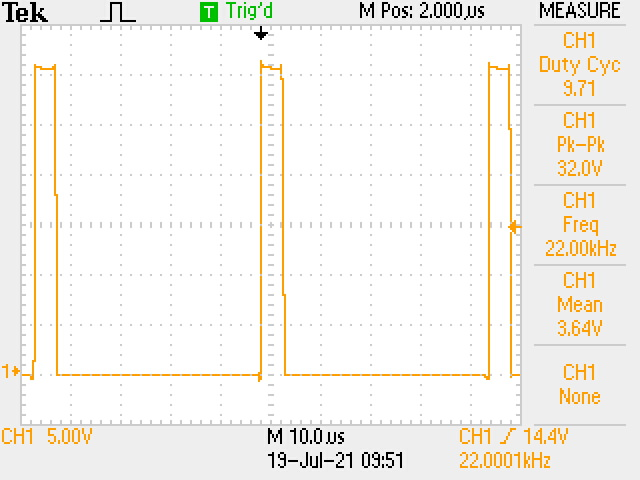
\includegraphics[width=0.8\textwidth]{high_side_drain_voltage.jpg}  
    \end{center}

    \item 

    From the efficiency vs output current plot below we can se that as the output current increases the efficiency will greatly increase, tapering off at 0.1mA. This lower efficiency at lower output currents will be due to the constant switching losses making up a larger portion of the total power output.

    \begin{center}
      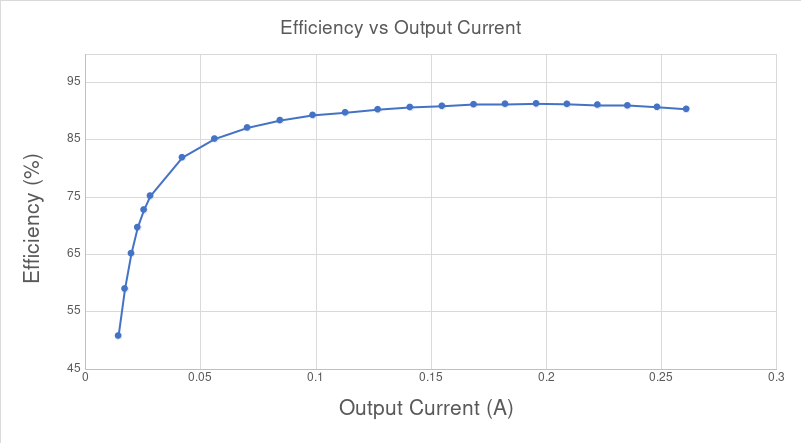
\includegraphics[width=0.8\textwidth]{effeciency.png}  
    \end{center}

    \item The bootstrap capacitor is used to help drive the high-side MOSFET. this is required as the source of this MOSFET is floating, meaning that we may not be able to provide the correct $V_{GS}$ to turn on the MOSFET. 

\end{enumerate}

\section*{Appendix}

\begin{enumerate}
  \item $ f = 22k\mathrm{Hz}, \;\;\; V_o = 20V, \;\;\; V_in=30V, \;\;\; R_L=100\Omega $
  \begin{align*}
    D\ &=\ \frac{V_{o}}{V_{in}} = 0.6\bar{6}\\
    I_{L}&=\frac{V_{o}}{R_{L}} = 0.2A\\
    I_{ripple}&=I_{L}\cdot0.4 = 0.24A\\\\
    L&=\frac{V_{o}\cdot\left(1-D\right)}{f\cdot I_{ripple}} = 3.7mH
  \end{align*}

  \item The converter will become discontinuous when the ripple current is twice the average inductor current, therefore we can rearrange for $f$:
  $$ f_{d}=\frac{V_{o}\cdot\left(1-D\right)}{L\cdot2I_{L}} = 4400\mathrm{Hz}$$

  \item I took the points of $(0\Omega , 0.4\mu s)$, $(200k\Omega , 5ns)$ and linearised, then re-arranged to find the resistance at $0.5\mu s$:
  $$ R_{D}=\frac{\left(D_{t}-0.4\right)\cdot200k}{5-0.4} = 4.373k\Omega$$
\end{enumerate}


\end{preview}
\end{document}